Two AlphaSense CO sensors were tested against the EPA reference.  The first sensor was 2.5 years old at the time of installation,  which ran for 38 days (from 4/15 to 5/23 2016 with one 40 minute service interruption).  The second sensor was 2 months old at the time of installation, and ran for 21 days (from 5/23 - 6/13 2016).  Our first test gave 55,589 minute-resolution samples to compare, our second test gave 30,150 samples.

These two tests give us a chance to compare manufacturer reliability and sensor aging effects.  The two datasets can also be combined after calibration to draw overall conclusions about the AlphaSense model CO-A4 sensor.  

\subsection{Pre-processing}

AlphaSense sensors give two main readings-- from an auxilary and a working electrode.  Additionally, they come with a calibration for sensitivity, as well as offset voltages for both electrodes.  The calibration function combines all of these using a non-linear temperature-dependent term (which scales the working electrode term differently over a few temperature ranges, linearly interpolated).  

While we used the provided calibration data to create one version of `corrected data', we've found from talking with faculty in the Environmental Engineering group that it is not uncommon for these laboratory based calibrations to drift substantially.  It is generally considered best practice to calibrate the sensors using co-location data.  The datasheet calibration provides results as seen in Figure \ref{fig:as_co_raw_zoomed}.

\begin{figure}[htb]
 	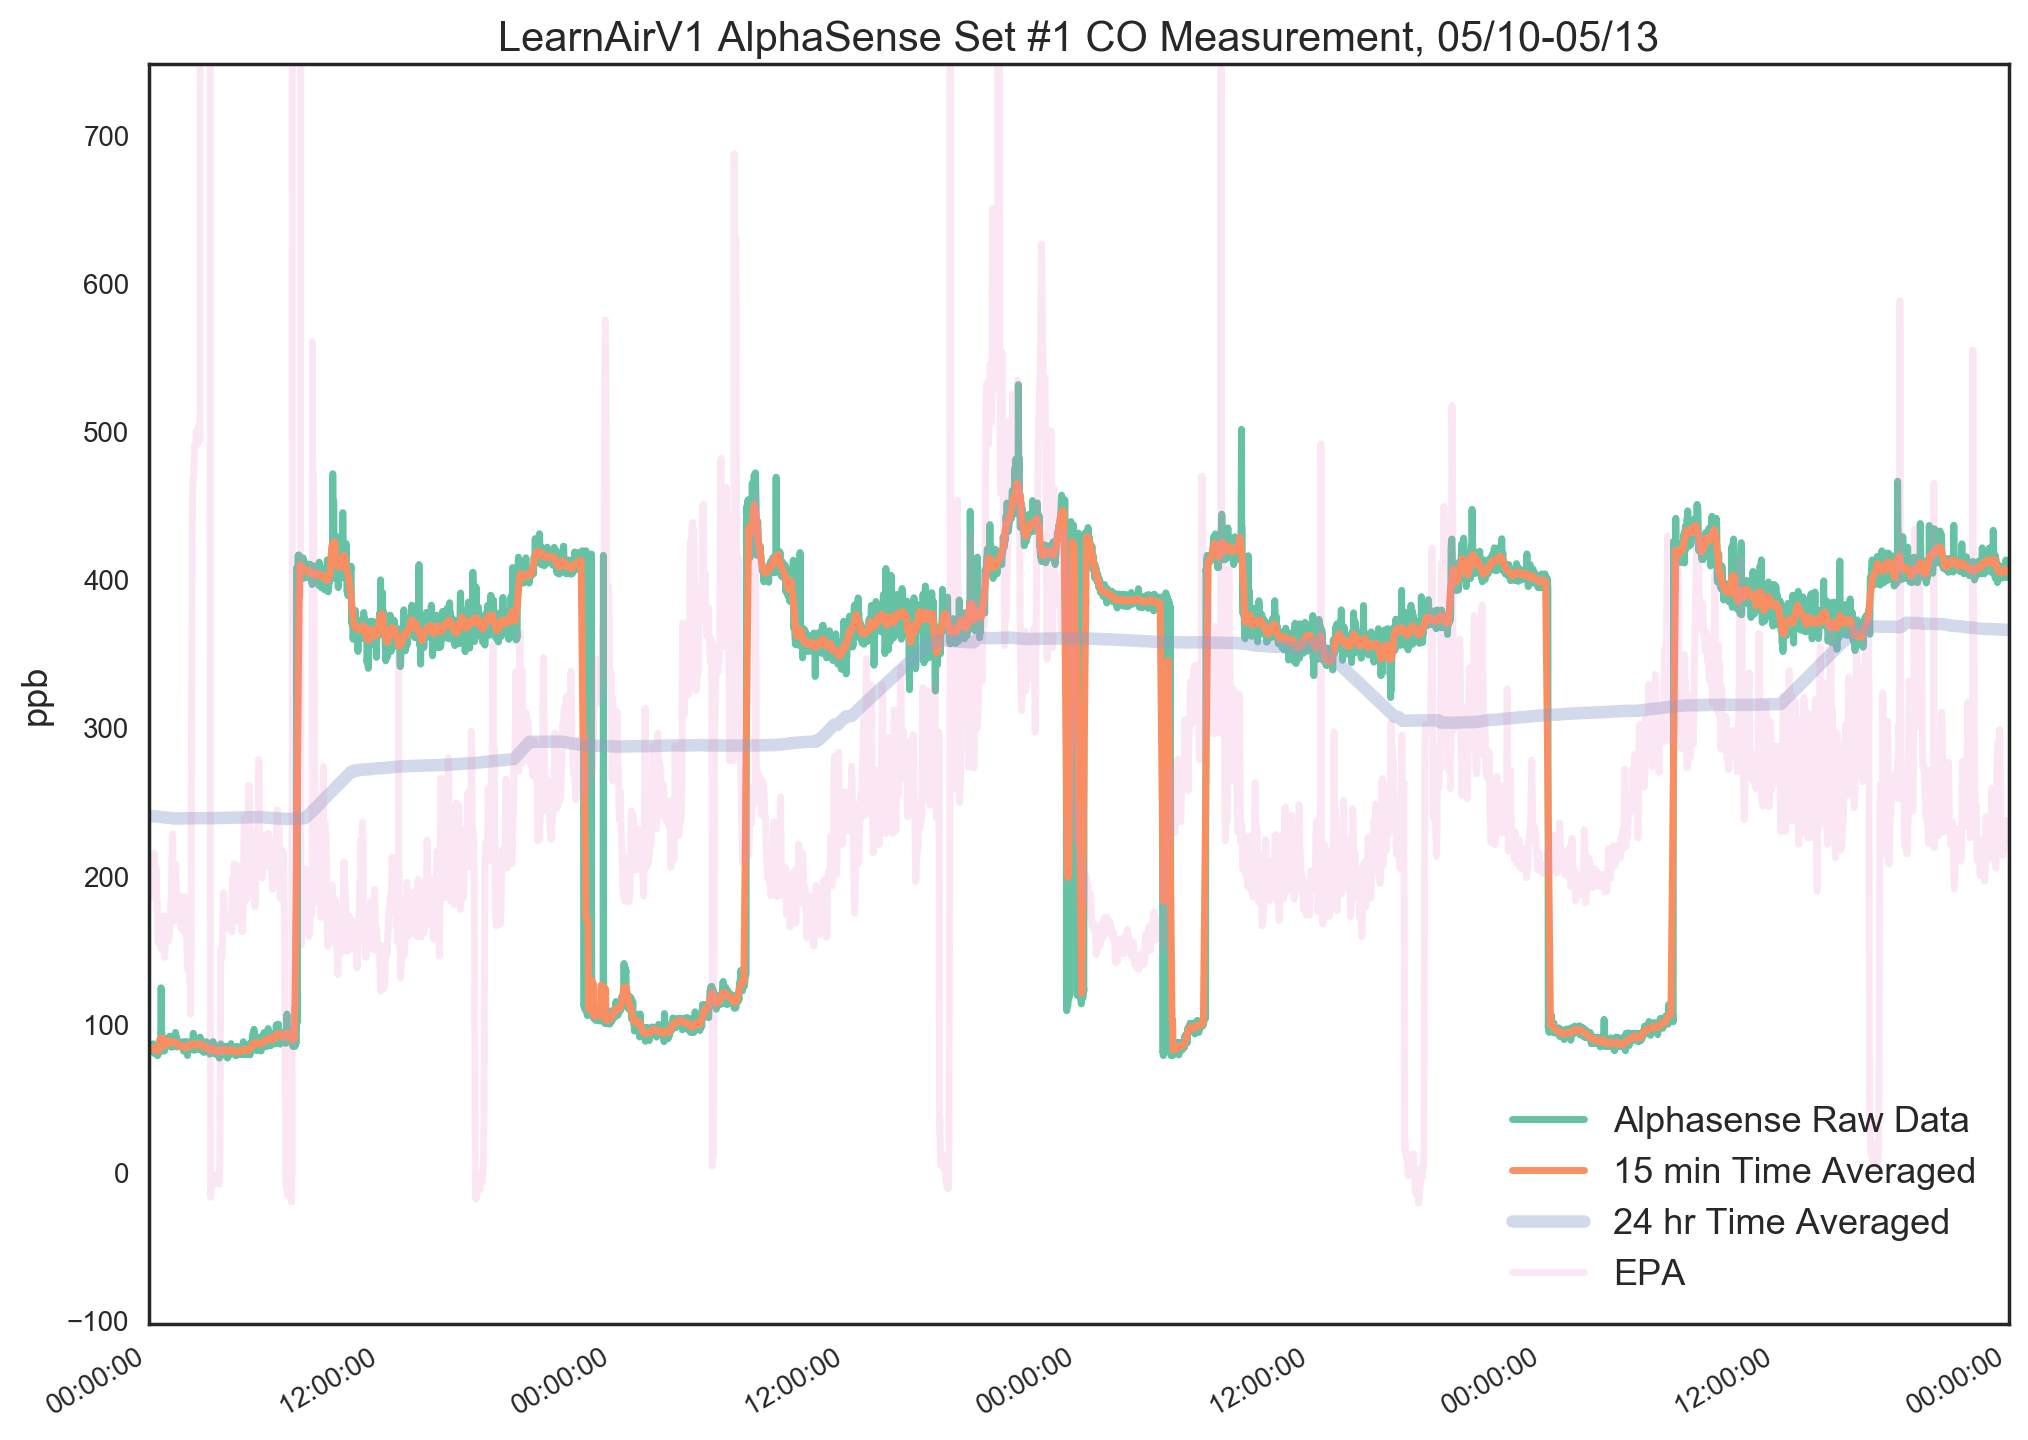
\includegraphics[width=\textwidth]{figs/as_co_raw_zoomed}               
 	 \caption{AlphaSense CO Sensor #1 Raw Data Zoomed}
  	\label{fig:as_co_raw_zoomed}
\end{figure}

One of the first things to notice is what appears to be quantization errors in the data.  This is not a result of the analog to digital conversion process on the Arduino-- we have a 5V, 10-bit input, which gives us 4.88 mV resolution.  Our sensor has around 0.3 mV/ppb sensitivity, so we expect our ADC to quantize the signal in ~16ppb steps.  The AlphaSense analog frontend board for the CO sensor is only capable of a 20 ppb noise level, so the limiting factor is not our ADC.  Examination of the raw Arduino data supports this assumption.  This `quantization' is actually the result of temperature dependent regimes in the calibration equation.  At 10, 20, and 30 degrees Celcius we enter different linear temperature correction regimes-- even though these are interpolated, the temperature dependence rapidly changes in a narrow span.

The proper way to `correct' these calibrations is worthy of a paper by itself.  Several techniques were attempted, mostly based on LMSE.  We tried basic scaling/offset the datasheet calibrated data as well as scaling/offset the data considering only one standard deviation of the mean for each sensor (in order to remove outliers).  We also attempted several more intuitive minimizations-- for instance, solving for a new sensitivity and offset voltages (using the actual calibration equation) seeded with the datasheet values.  Additionally, we tried minimizing by solving for new temperature dependence terms, in case the actual thresholds or scale factors were shifted slightly.  Finally, we tried non-standard minimization strategies-- setting thresholds for the values that are part of the cost minimization calculation, and using absolute error (since LMSE penalizes larger errors more, and we really want to ignore the larger errors without incentivizing a cost function to create larger errors).

In general, the high frequency trends and sensitivity of the sensor are very in line with real pollutant concentration.  The large, nearly step-wise variations due to temperature compensation seem to be the biggest issue with close tracking of the actual data.  Most LMSE techniques aimed specifically at this temperature dependence completely eliminated the behavior-- while this tracks the real signal better, it also gives a less dynamic signal with an unrealistic underlying assumption (that the sensor actually has \textit{no} temperature dependence).  With a more thorough understanding of how these sensors age and change, it may be easier to design an intuitive minimization for better calibration.  For the purposes of this test (and the tests with other AlphaSense gas sensors), we minimized error by solving for new electrode offset voltages only.  The results of this strategy for both the older and newer sensors can be seen in Figures \ref{fig:as2_co_lmse} and \ref{fig:as_co_with_5_accuracy_zoomed}.

\begin{figure}[htb]
 	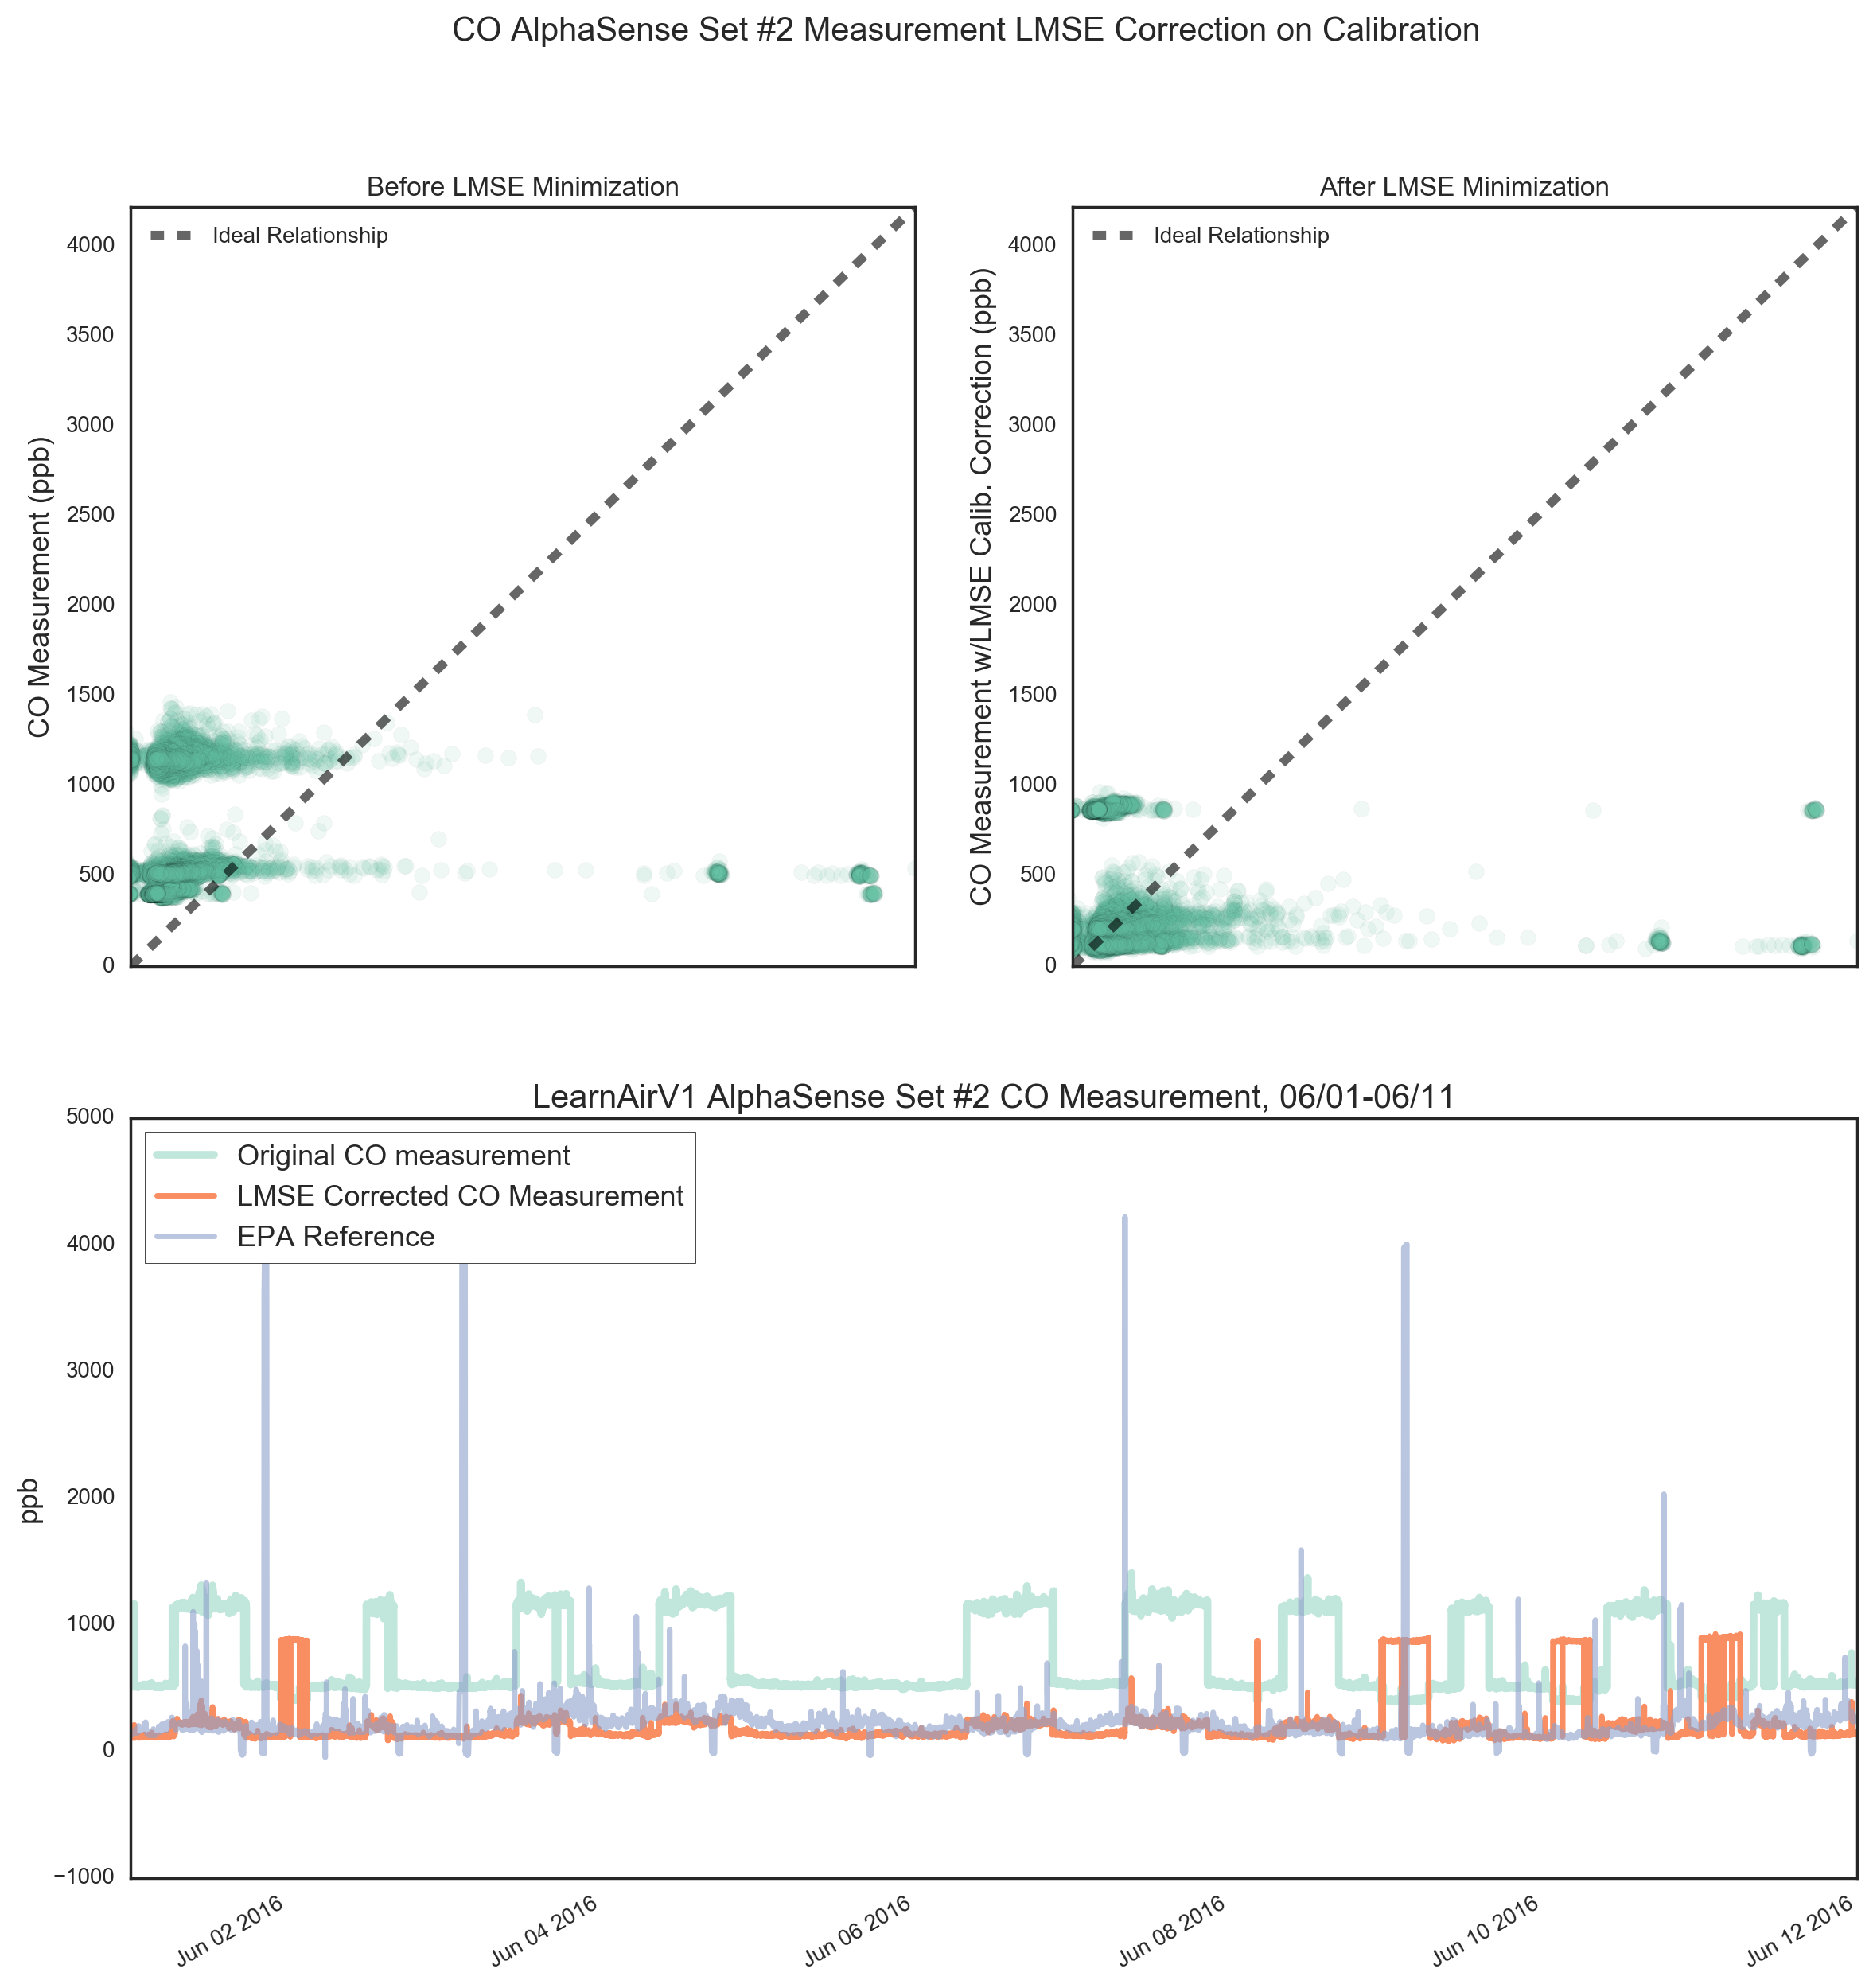
\includegraphics[width=\textwidth]{figs/as2_co_lmse}               
 	 \caption{AlphaSense CO Sensor #2 after LMSE Calibration}
  	\label{fig:as2_co_lmse}
\end{figure}

\subsection{Machine Learning}

Both sensors were treated independently to start, and their output was compared.  Agreement between the two can provide us with high confidence about underlying mechanisms.  Both were optimized using a grid based parameter search of C = [0.001, 0.1, 10, 1000] and penalty-type=['L1', 'L2'] with a 2-fold cross-validation.  Both gave the same optimum model using an L1 penalty and C=1000.  The older sensor gave an AUC-ROC of 0.89, while the newer one gave 0.90.  Figure \ref{fig:as_co_with_5_accuracy_zoomed} shows the comparison of the reference with our calibrated data, using a 5\% tolerance (around $\pm$100 ppb, a relatively ambitious tolerance).   

\begin{figure}[htb]
 	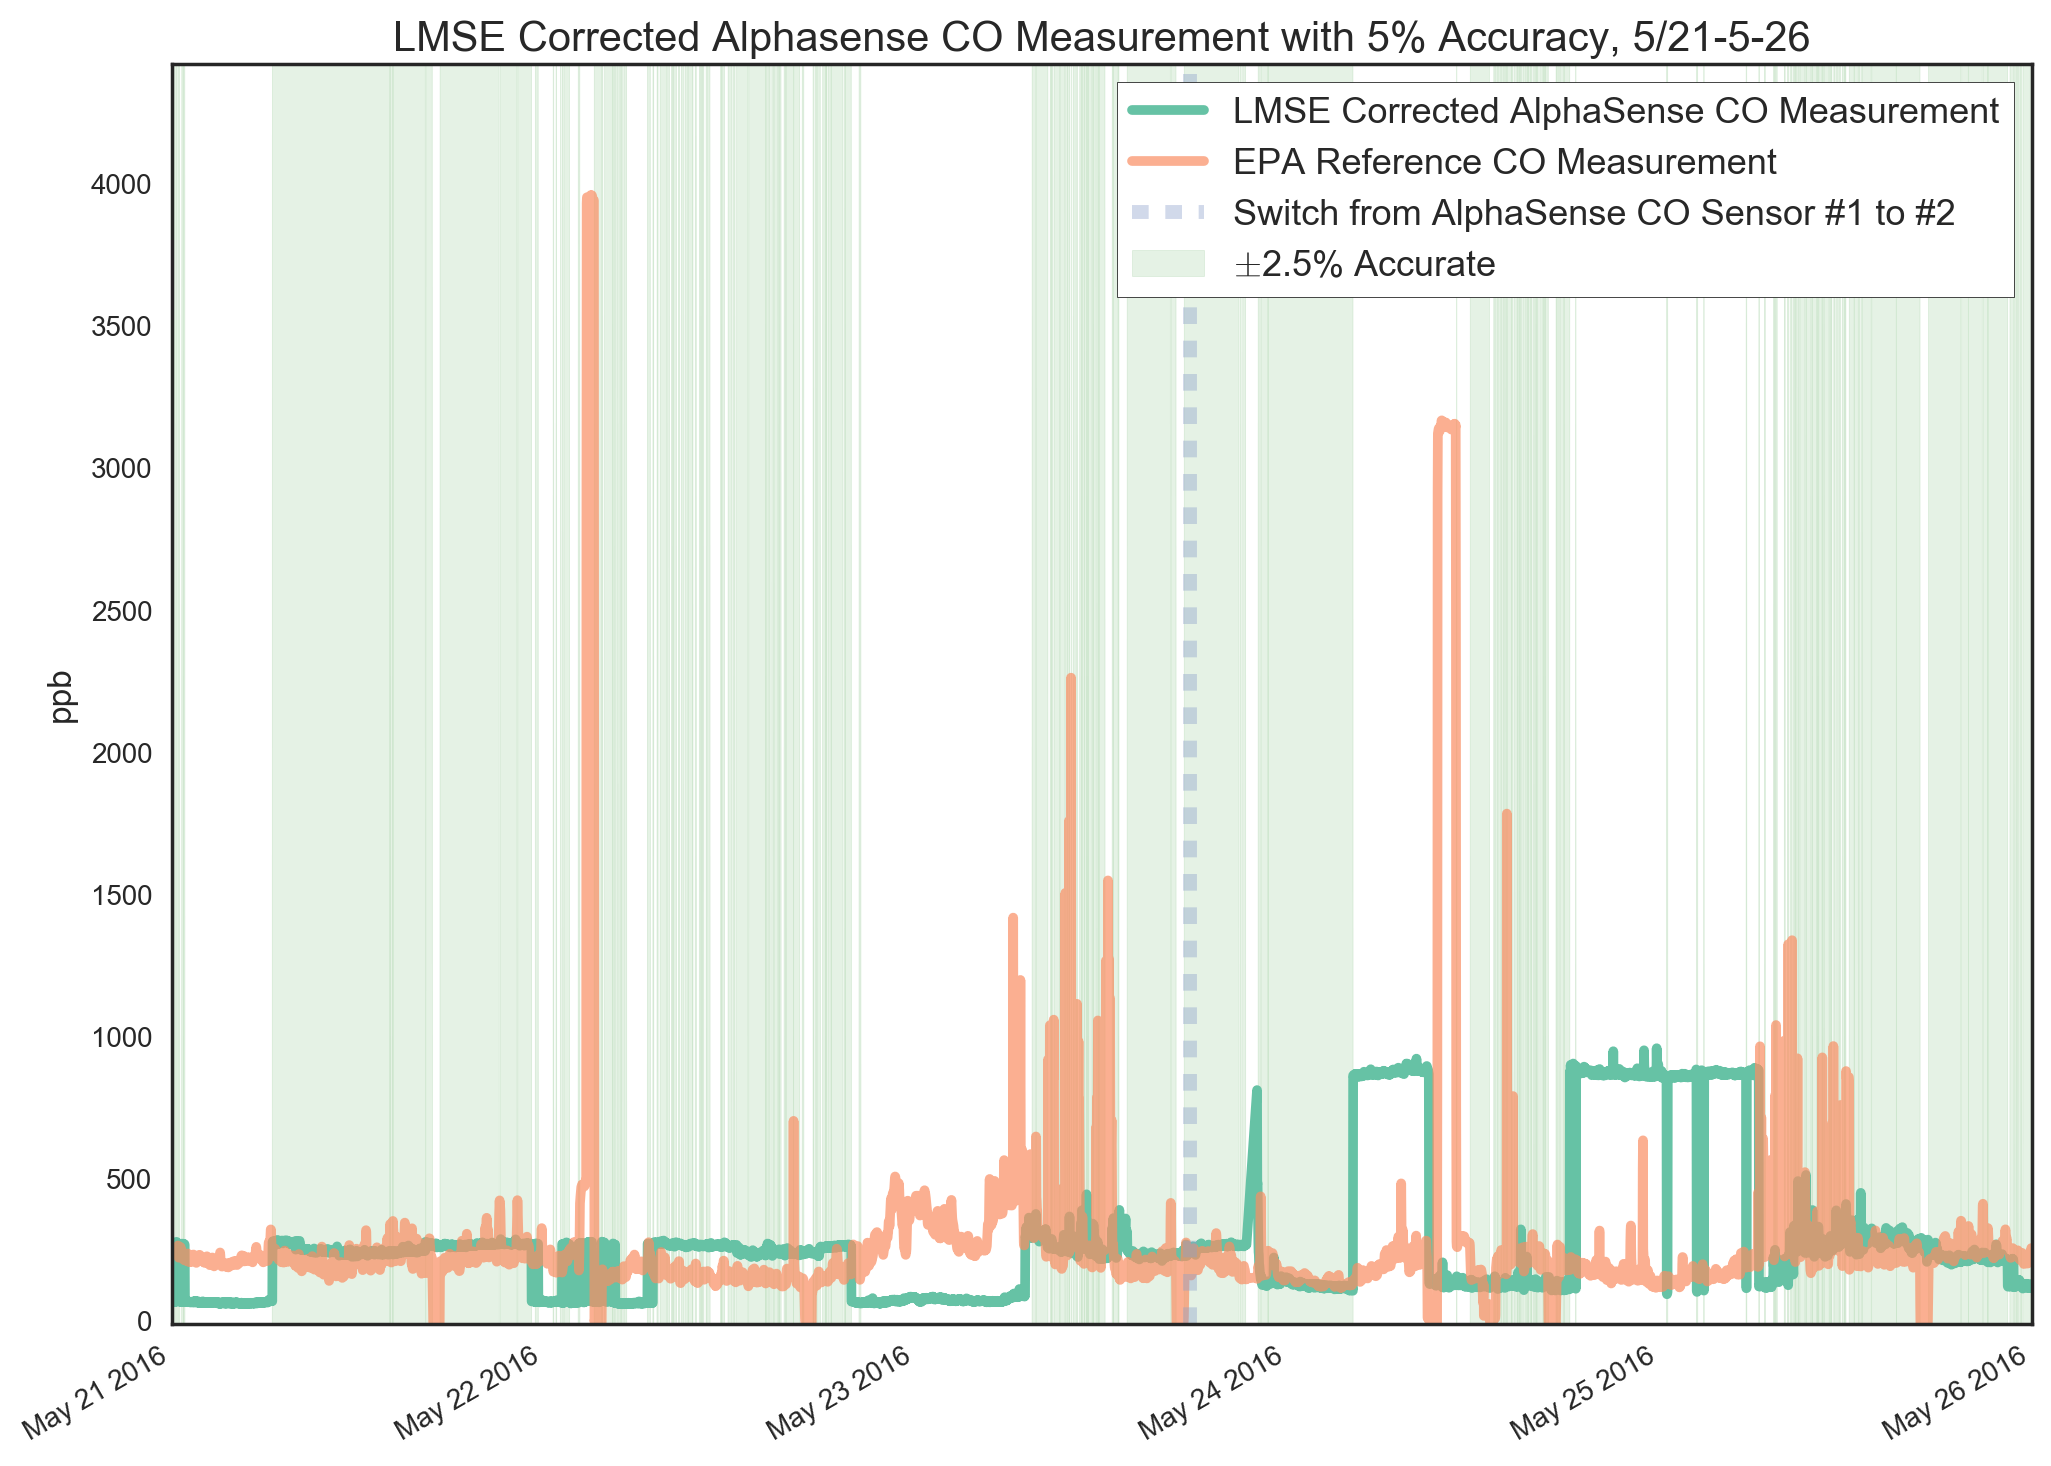
\includegraphics[width=\textwidth]{figs/as_co_with_5_accuracy_zoomed}               
 	 \caption{AlphaSense CO Sensor #1 and #2 with 5\% Accuracy Threshold}
  	\label{fig:as_co_with_5_accuracy_zoomed}
\end{figure}

The error rates of table \ref{tab:as1_co_error_rates} and \ref{tab:as2_co_error_rates} show relatively robust behavior from the entire feature set to just the top fifteen.  The older sensor has slightly elevated error rates compared to the newer one, but it also saw more dynamic weather conditions.  High variability in the chunked error rates suggests we haven't trained on enough data yet.
\floatbarrier

\begin{table}[]
\centering
\begin{tabular}{|c|c|c|c|c|}
\toprule
\multicolumn{5}{|c|}{Error Rates for CO Sensor #1 with Logistic Regression} \\
&\multicolumn{2}{|c|}{all features} & \multicolumn{2}{|c|}{top 15 features} \\
&shuffled & chunked & shuffled & chunked \\
avg & 0.18 & 0.21 & 0.20 & 0.20 \\
min & 0.17 & 0.17 & 0.19 & 0.12 \\
max & 0.18 & 0.28 & 0.20 & 0.28 \\
\bottomrule
\end{tabular}
\label{tab:as1_co_error_rates}
\caption{Error Rates for Predicting CO Sensor #1 Accuracy with Logistic Regression}
\end{table}

\begin{table}[]
\centering
\begin{tabular}{|c|c|c|c|c|}
\toprule
\multicolumn{5}{|c|}{Error Rates for CO Sensor #2 with Logistic Regression} \\
&\multicolumn{2}{|c|}{all features} & \multicolumn{2}{|c|}{top 15 features} \\
&shuffled & chunked & shuffled & chunked \\
avg & 0.14 & 0.20 & 0.16 & 0.17 \\
min & 0.13 & 0.10 & 0.15 & 0.11 \\
max & 0.14 & 0.28 & 0.16 & 0.22 \\
\bottomrule
\end{tabular}
\label{tab:as2_co_error_rates}
\caption{Error Rates for Predicting CO Sensor #2 Accuracy with Logistic Regression}
\end{table}
\floatbarrier


\begin{margintable}[-2cm]
\centering
\offinterlineskip
\hspace*{-5cm}\raisebox{-4cm}[0pt][0pt]{\rotatebox[origin=c]{90}{\parbox[c][0pt][c]{3cm}{\textbf{Actual Values}\\[20pt]}}}\par
\hspace{.3cm}\MyHBox[\marginparwidth]{Predicted Values}\par
\vspace{-.5cm}
\hspace*{1cm}\MyHBox{0}\MyHBox{1}\par
\MyTBox{0}{4751.0}{943.0}
\vspace{-.35cm}\MyTBox{1}{1023.4}{4400.4}\raisebox{-1cm}
}
\label{tab:as1_co_confusion}
\caption{Average AlphaSense CO Sensor #1 Confusion Matrix w/Shuffled K-Fold}
\end{margintable}


Despite the larger error rates, our AUC-ROC curves show reasonably good results-- 0.89-0.90 for the shuffled, and  0.69-0.91 for the chunked.  This is slightly better for the second, newer sensor (0.90-0.91 and 0.72-0.91).  The results are thus quite promising in their predictive merit.

When we reduce the feature set to 15 features, we drop in accuracy to the mid- to high- 0.8s, but the agreement across sensors and across chunked and shuffled strategies is the highest we've seen so far.  This stands out as a reasonably well executed model-- it has verified predictive value, and it appears to agree with itself across season and across sensor.  The top features-- the sensor itself, NO2, black carbon, humidity, temperature, and windspeed-- are all common sense candidates for this type of sensor.  

\begin{margintable}[]
\centering
\offinterlineskip
\hspace*{-5cm}\raisebox{-4cm}[0pt][0pt]{\rotatebox[origin=c]{90}{\parbox[c][0pt][c]{3cm}{\textbf{Actual Values}\\[20pt]}}}\par
\hspace{.3cm}\MyHBox[\marginparwidth]{Predicted Values}\par
\vspace{-.5cm}
\hspace*{1cm}\MyHBox{0}\MyHBox{1}\par
\MyTBox{0}{1326.2}{623.0}
\vspace{-.35cm}\MyTBox{1}{200.4}{3880.4}\raisebox{-1cm}
}
\label{tab:as2_co_confusion}
\caption{Average AlphaSense CO Sensor #2 Confusion Matrix w/Shuffled K-Fold}
\end{margintable}



\begin{figure}[htb]
 	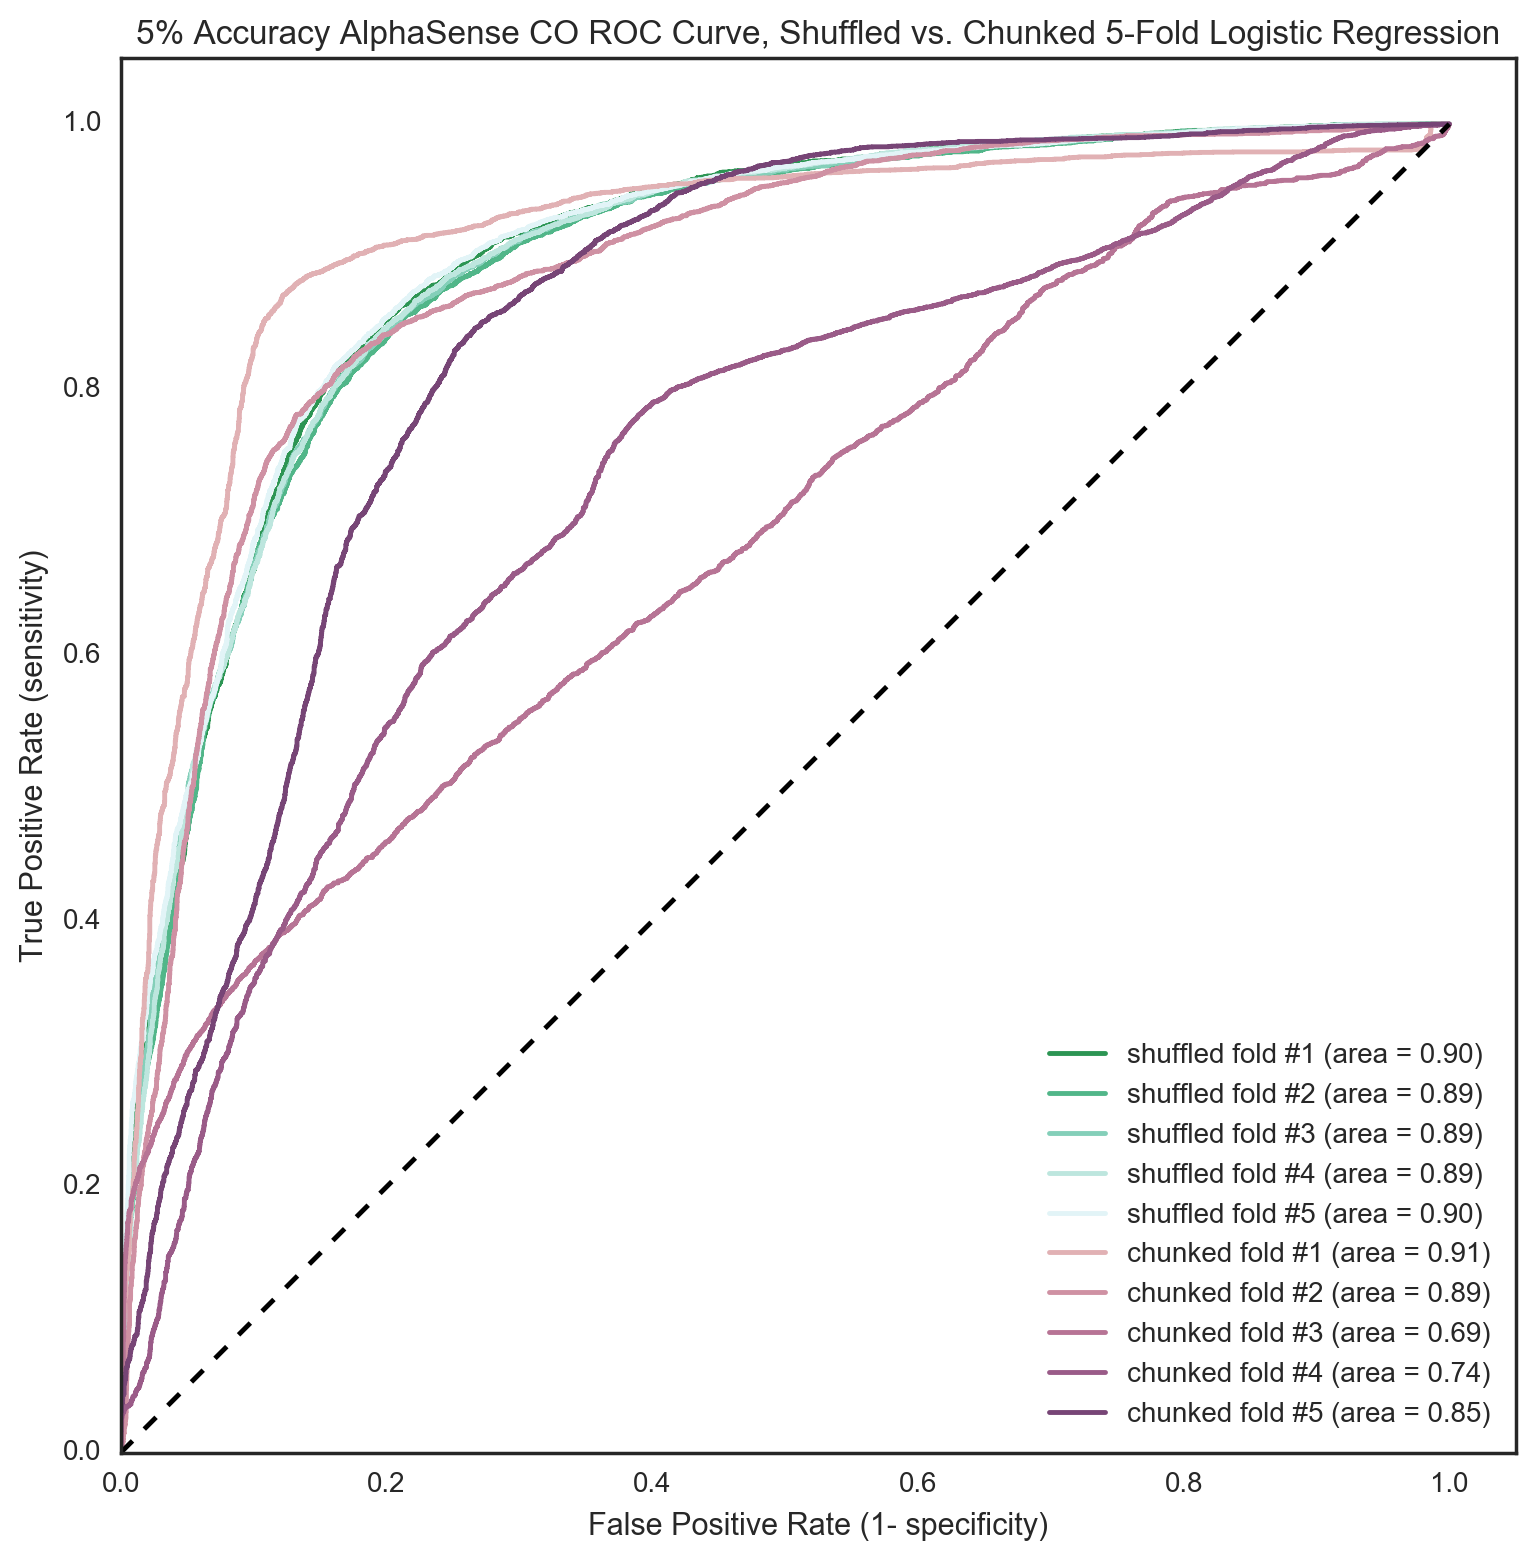
\includegraphics[width=\textwidth-1cm]{figs/as1_co_5_roc}               
 	 \caption{AlphaSense CO Sensor #1 ROC Curve}
  	\label{fig:as1_co_5_roc}
\end{figure}


\begin{figure}[htb]
 	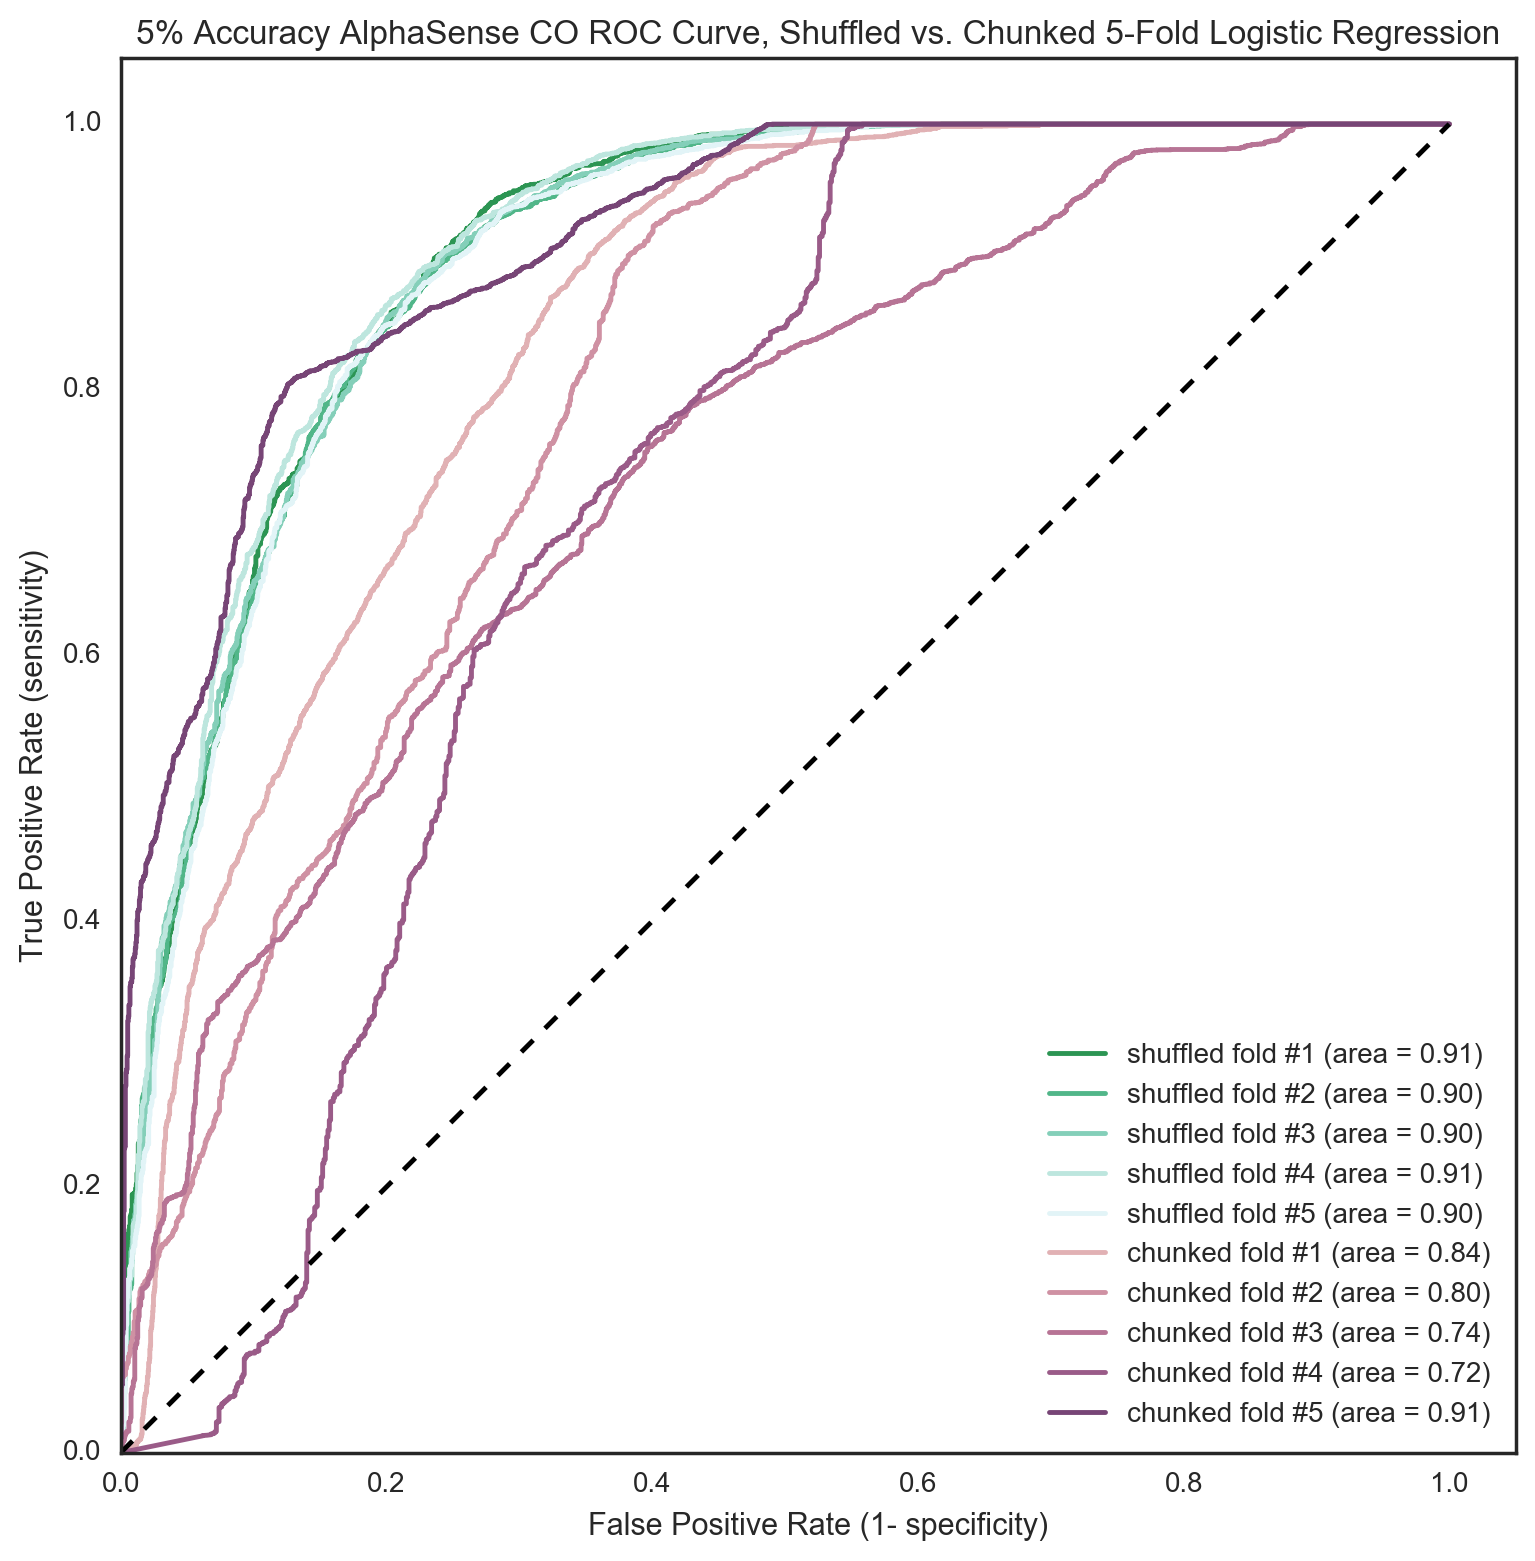
\includegraphics[width=\textwidth-1cm]{figs/as2_co_5_roc}               
 	 \caption{AlphaSense CO Sensor #2 ROC Curve}
  	\label{fig:as2_co_5_roc}
\end{figure}

See Appendix D for more plots outlining the raw data, more information on the models with different accuracy thresholds and averaging, plots of the data with a correct/incorrect prediction overlay, and the Random Tree reduced-feature selection table and corresponding ROC curves. 

\begin{table}
\centering
\small
\begin{tabular}{lllllllll}
\\
\\
\toprule
     & Corr. & Lasso & Lin Reg & RF   & RFE  & Ridge & Stability & Mean \\
\midrule
as\_co                                        & 0.95  & 0.29  & 0          & 1    & 0.64 & 0     & 0.51      & 0.48 \\
lmse\_calib\_as\_co                           & 0.95  & 0     & 0          & 0.68 & 0.65 & 0     & 0.59      & 0.41 \\
avg\_60\_forecastio\_humidity                 & 0.29  & 0     & 0.01       & 0.03 & 1    & 0.73  & 0.59      & 0.38 \\
forecastio\_wind                              & 0     & 0     & 0.05       & 0    & 0.76 & 0.54  & 1         & 0.34 \\
sck\_temperature                              & 0.92  & 0     & 0          & 0.02 & 0.98 & 0     & 0.44      & 0.34 \\
alphaS2\_work                                 & 0     & 1     & 0          & 0.02 & 0.25 & 0.01  & 1         & 0.33 \\
alphaTemp                                     & 0.94  & 0     & 0          & 0    & 0.92 & 0     & 0.48      & 0.33 \\
as\_temperature                               & 0.94  & 0     & 0          & 0    & 0.91 & 0     & 0.46      & 0.33 \\
humidity\_box\_differential                   & 0.14  & 0     & 0.01       & 0.04 & 1    & 0.73  & 0.37      & 0.33 \\
avg\_15\_as\_temperature                      & 0.99  & 0     & 0          & 0.02 & 0.57 & 0.16  & 0.49      & 0.32 \\
avg\_720\_lmse\_scaled\_sharpDust             & 0.02  & 0     & 0          & 0.03 & 0.54 & 1     & 0.68      & 0.32 \\
Temperature ( C RAW)                          & 0.92  & 0.07  & 0          & 0.02 & 0.63 & 0     & 0.45      & 0.3  \\
Solar Panel ( V)                              & 0.14  & 0     & 1          & 0    & 0.95 & 0     & 0         & 0.3  \\
forecastio\_temperature                       & 0.68  & 0.09  & 0          & 0    & 0.87 & 0     & 0.37      & 0.29 \\
avg\_60\_forecastio\_temperature\_c           & 0.7   & 0     & 0          & 0.03 & 0.97 & 0.09  & 0.25      & 0.29 \\
evening                                       & 0.02  & 0     & 0.1        & 0.02 & 0.99 & 0.04  & 0.81      & 0.28 \\
night                                         & 0.18  & 0     & 0.05       & 0    & 1    & 0.11  & 0.59      & 0.28 \\
day                                           & 0.18  & 0     & 0.05       & 0    & 0.96 & 0.11  & 0.6       & 0.27 \\
forecastio\_temperature\_c                    & 0.68  & 0     & 0          & 0    & 0.88 & 0     & 0.31      & 0.27 \\
morning                                       & 0.01  & 0     & 0.1        & 0    & 1    & 0.12  & 0.61      & 0.26 \\
avg\_60\_forecastio\_cloudCover               & 0     & 0     & 0          & 0.04 & 0.48 & 0.29  & 1         & 0.26 \\
forecastio\_humidity                          & 0.28  & 0     & 0          & 0    & 0.55 & 0.26  & 0.69      & 0.25 \\
derivative\_avg\_720\_lmse\_scaled\_sharpDust & 0     & 0     & 0          & 0.01 & 0.61 & 0.15  & 1         & 0.25 \\
hour\_of\_day                                 & 0.02  & 0.41  & 0          & 0.01 & 0.22 & 0.01  & 1         & 0.24\\
\bottomrule
\end{tabular}
\label{tab:as1_co_top_features}
\caption{Top Features for Predicting AlphaSense CO Sensor #1}
\end{table}





\begin{table}
\centering
\small
\begin{tabular}{lllllllll}
\\
\\
\toprule
     & Corr. & Lasso & Lin Reg & RF   & RFE  & Ridge & Stability & Mean \\
\midrule
lmse\_calib\_as\_co                            & 1     & 0.1   & 0          & 1    & 0.18 & 0     & 1         & 0.47 \\
evening                                        & 0     & 0     & 0.01       & 0.01 & 0.96 & 0.04  & 0.99      & 0.29 \\
avg\_60\_forecastio\_windSpeed                 & 0.3   & 1     & 0          & 0.15 & 0.06 & 0     & 0.55      & 0.29 \\
Solar Panel ( V)                               & 0.11  & 0     & 1          & 0    & 0.86 & 0     & 0         & 0.28 \\
forecastio\_windSpeed                          & 0.27  & 0.62  & 0          & 0.02 & 0.29 & 0.01  & 0.72      & 0.28 \\
sck\_humidity\_saturated                       & 0.05  & 0     & 0          & 0    & 0.59 & 1     & 0.33      & 0.28 \\
avg\_15\_as\_no2                               & 0.4   & 0.29  & 0          & 0.01 & 0.73 & 0     & 0.36      & 0.26 \\
forecastio\_fog                                & 0.11  & 0     & 0.71       & 0    & 0.94 & 0     & 0         & 0.25 \\
as\_o3                                         & 0.41  & 0.08  & 0          & 0.01 & 0.72 & 0     & 0.5       & 0.25 \\
derivative\_avg\_1440\_lmse\_scaled\_sharpDust & 0.14  & 0     & 0          & 0.01 & 0.6  & 0.03  & 0.99      & 0.25 \\
as\_no2                                        & 0.41  & 0     & 0          & 0    & 0.71 & 0.01  & 0.53      & 0.24 \\
lmse\_as\_no2                                  & 0.41  & 0     & 0          & 0    & 0.73 & 0     & 0.48      & 0.23 \\
lmse\_avg\_15\_as\_no2                         & 0.4   & 0     & 0.01       & 0.01 & 0.81 & 0     & 0.41      & 0.23 \\
bkcarbon                                       & 0.05  & 0     & 0          & 0.13 & 0.5  & 0.1   & 0.81      & 0.23 \\
avg\_15\_derivative\_sck\_temperature          & 0     & 0     & 0          & 0.01 & 0.57 & 0.41  & 0.53      & 0.22 \\
daily\_avg\_forecastio\_temperature            & 0.22  & 0     & 0          & 0.03 & 0.45 & 0.1   & 0.71      & 0.22 \\
avg\_15\_lmse\_as\_no2                         & 0.4   & 0     & 0.01       & 0.01 & 0.82 & 0     & 0.3       & 0.22 \\
derivative\_avg\_360\_lmse\_as\_no2            & 0     & 0     & 0          & 0.02 & 0.59 & 0.31  & 0.62      & 0.22 \\
avg\_60\_bkcarbon                              & 0.06  & 0     & 0          & 0.07 & 0.55 & 0.15  & 0.73      & 0.22 \\
afternoon                                      & 0.13  & 0     & 0.01       & 0    & 0.97 & 0.06  & 0.31      & 0.21 \\
avg\_720\_bkcarbon                             & 0.02  & 0     & 0          & 0.18 & 0.53 & 0.06  & 0.69      & 0.21 \\
alphaS2\_work                                  & 0.02  & 0.61  & 0          & 0.03 & 0.23 & 0.02  & 0.49      & 0.2  \\
avg\_60\_as\_no2                               & 0.39  & 0.01  & 0          & 0.02 & 0.99 & 0     & 0         & 0.2  \\
avg\_15\_lmse\_calib\_as\_co                   & 0.94  & 0     & 0          & 0.05 & 0.05 & 0     & 0.35      & 0.2 \\
\bottomrule
\end{tabular}
\label{tab:as2_co_top_features}
\caption{Top Features for Predicting AlphaSense CO Sensor #2}
\end{table}